\chapter{Advanced Algorithms}
\label{chap:advanced_algorithms}

\begin{figure}[ht]
	\hfill
	\begin{minipage}{0.5\textwidth}
		\centering
		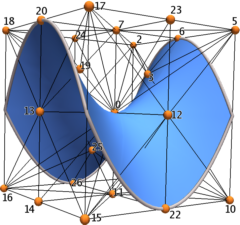
\includegraphics{VTKTextbook-168}
		\caption*{\texttt{An isocontour of a tri--quadratic Lagrange--interpolantion. Image courtesy D. Thompson and P. Pébay Sandia National Labs.}}
	\end{minipage}
\end{figure}

\firstletter{W}e return again to visualization algorithms.
This chapter describes algorithms that are either more complex to implement, or less widely used for 3D visualization applications.
We retain the classification of algorithms as either scalar, vector, tensor, or modelling algorithms.

\section{Scalar Algorithms}

As we have seen, scalar algorithms often involve mapping scalar values through a lookup table, or creating contour lines or surfaces.
In this section, we examine another contouring algorithm, dividing cubes , which generates contour surfaces using dense point clouds.
We also describe carpet plots.
Carpet plots are not true 3D visualization techniques, but are widely used to visualize many types of scalar data.
Finally, clipping is another important algorithm related to contouring, where cells are cut into pieces as a function of scalar value.

\subsection{Dividing Cubes}

\begin{figure}[!htb]
    \centering
    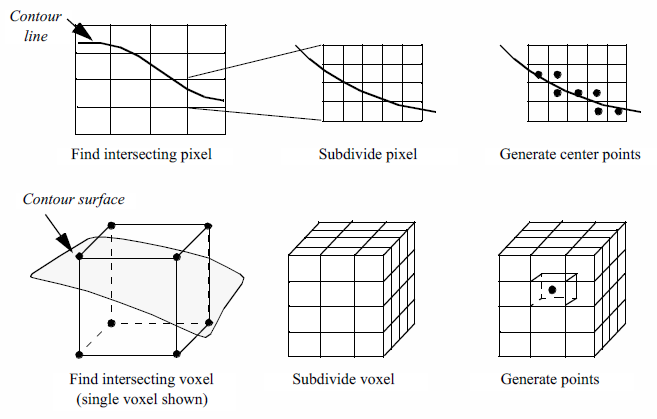
\includegraphics[width=0.98\textwidth]{Figure9-1}\\
    \caption{Overview of the dividing cubes algorithm. Voxels through which the contour passes are subdivided into subvoxels at less than screen resolution. If the contour passes through a subvoxel, a center point is generated.}\label{fig:Figure9-1}
\end{figure}


\begin{figure}[!htb]
    \centering
    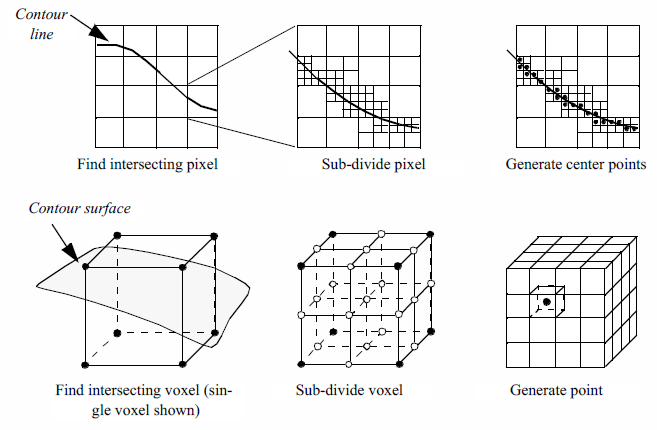
\includegraphics[width=0.98\textwidth]{Figure9-2}\\
    \caption{Recursive dividing cubes algorithm. Top half of figure shows algorithm depicted in two dimensions. Lower half depicts algorithm in three dimensions.}\label{fig:Figure9-2}
\end{figure}


\section{Vector Algorithms}

\subsection{Vector Field Topology}

\begin{figure}[htb]
	\begin{subfigure}[h]{0.32\linewidth}
		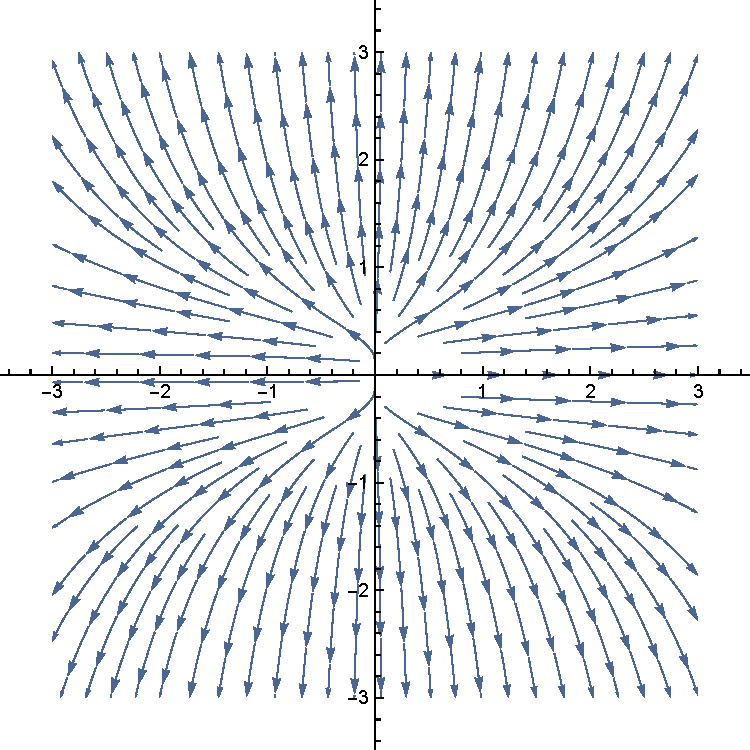
\includegraphics[width=0.86\linewidth]{Figure9-13a}
		\captionsetup{justification=centering}
		\caption*{Repelling Node\\$R_1, R_2 > 0$\\$I_1, I_2 = 0$}
		\label{fig:Figure9-13a}
	\end{subfigure}
	\hfill
	\begin{subfigure}[h]{0.32\linewidth}
		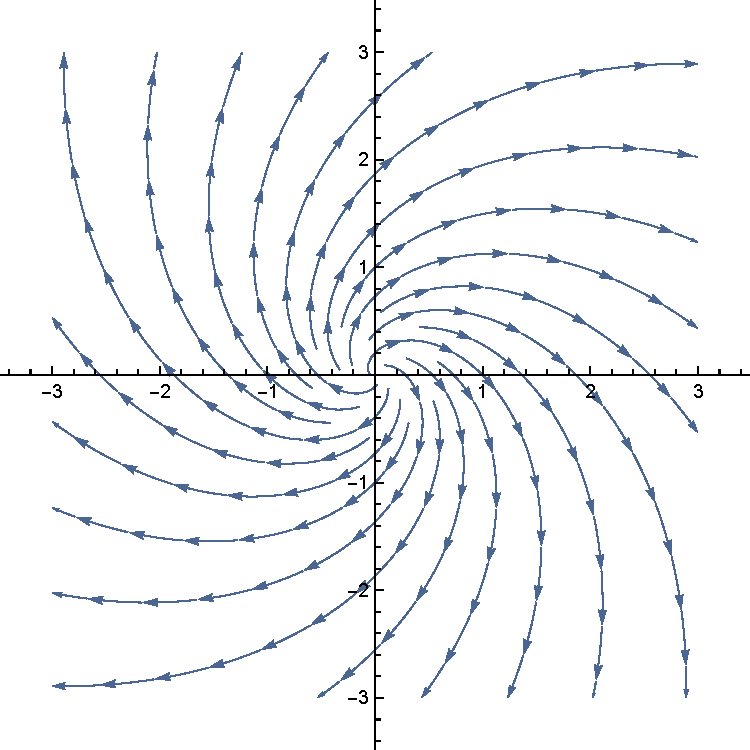
\includegraphics[width=0.86\linewidth]{Figure9-13b}
		\captionsetup{justification=centering}
		\caption*{Repelling Focus\\$R_1, R_2 > 0$\\$I_1, I_2 \neq 0$}
		\label{fig:Figure9-13b}
	\end{subfigure}
	\hfill
	\begin{subfigure}[h]{0.32\linewidth}
		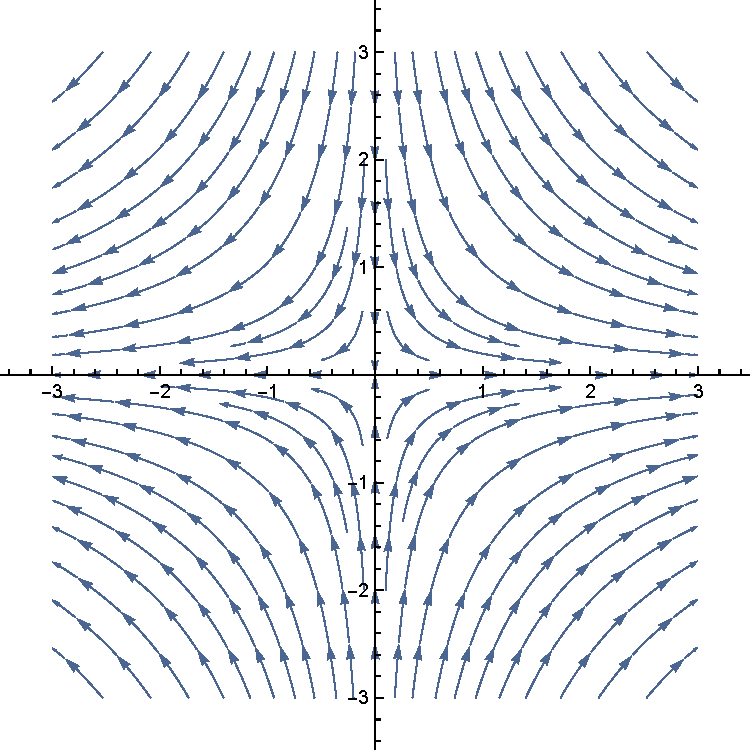
\includegraphics[width=0.86\linewidth]{Figure9-13c}
		\captionsetup{justification=centering}
		\caption*{Saddle Point\\$R_1 \times R_2 < 0$\\$I_1, I_2 = 0$}
		\label{fig:Figure9-13c}
	\end{subfigure}
	\hfill
		\begin{subfigure}[h]{0.32\linewidth}
		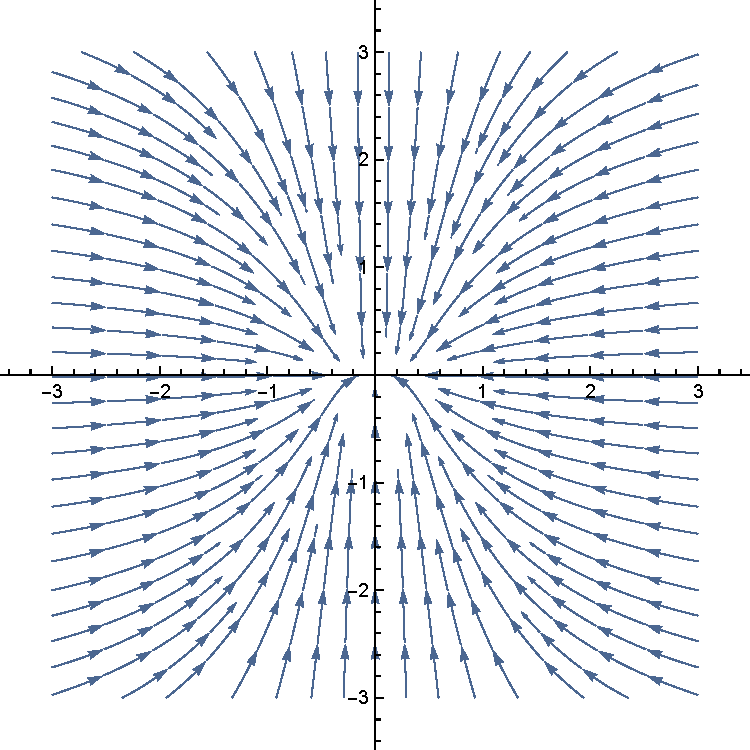
\includegraphics[width=0.86\linewidth]{Figure9-13d}
		\captionsetup{justification=centering}
		\caption*{Attracting Node\\$R_1, R_2 < 0$\\$I_1, I_2 = 0$}
		\label{fig:Figure9-13d}
	\end{subfigure}
	\hfill
	\begin{subfigure}[h]{0.32\linewidth}
		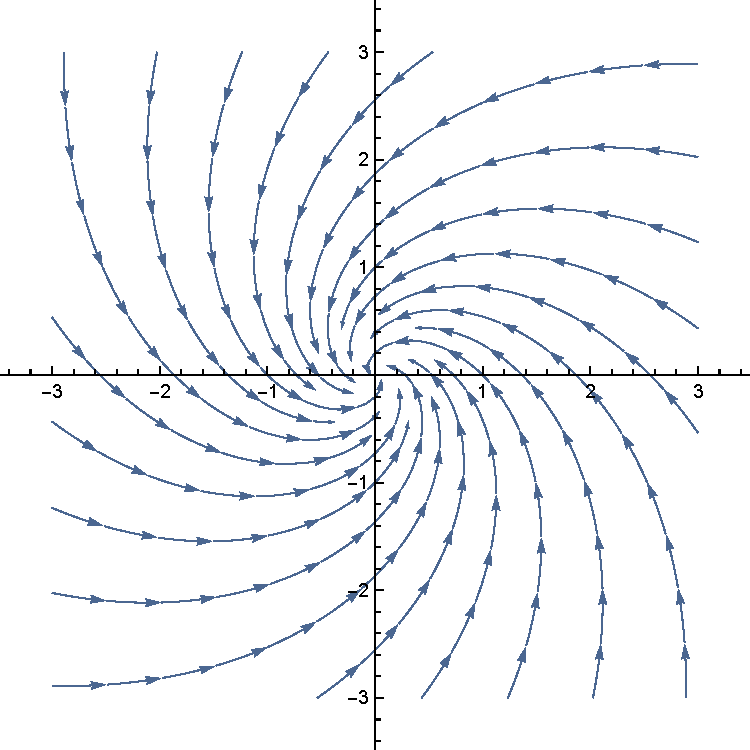
\includegraphics[width=0.86\linewidth]{Figure9-13e}
		\captionsetup{justification=centering}
		\caption*{Attracting Focus\\$R_1, R_2 < 0$\\$I_1, I_2 \neq 0$}
		\label{fig:Figure9-13e}
	\end{subfigure}
	\hfill
	\begin{subfigure}[h]{0.32\linewidth}
		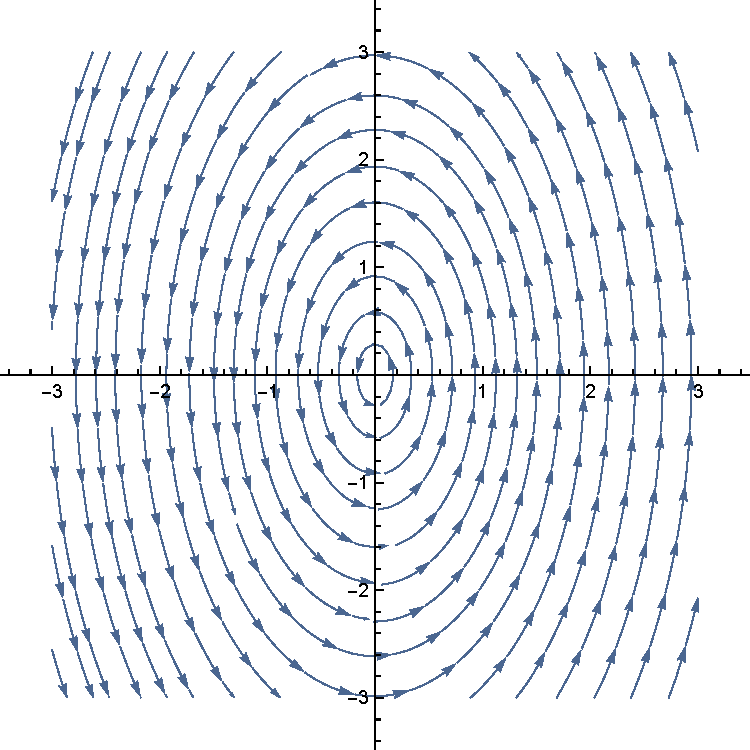
\includegraphics[width=0.86\linewidth]{Figure9-13f}
		\captionsetup{justification=centering}
		\caption*{Center\\$R_1, R_2 = 0$\\$I_1, I_2 \neq 0$}
		\label{fig:Figure9-13f}
	\end{subfigure}
	\caption{Critical points in two dimensions. The real part of the eigenvalues ($R_1$, $R_2$) of the matrix of first derivatives control the attraction or repulsion of the vector field. The imaginary part of the eigenvalues ($I_1$, $I_2$) controls the rotation.}\label{fig:Figure9-13}
\end{figure}


\begin{equation}\label{eq:9.12}
H_d = \overrightarrow{v\ } \cdot \overrightarrow{w\ } = \vert \overrightarrow{v\ } \vert \vert \overrightarrow{w\ } \vert \cos(\phi)
\end{equation}
\myequations{Scalar function of the vector dot product. }

\section{Tensor Algorithms}

\section{Modelling Algorithms}

\subsection{Decimation}

\begin{description}
	\item[Triangulation.] \label{subsec:decimation.triangulation} After deleting a point, the resulting hole must be retriangulated.
\end{description}

\subsection{Mesh Smoothing}
\label{subsec:mesh_smoothing}

\subsection{Visualizing Unstructured Points}
\label{subsec:visualizing_unstructured_points}

\subsection{Texture Algorithms}
\label{subsec:texture_algorithms}

\section{Putting It All Together}

\subsection{Connectivity}
\label{subsec:connectivity}

\section{ Bibliographic Notes}

Dividing cubes is an interesting algorithm because of the possibilities it suggests \cite{Cline88}. Point primitives are extremely simple to render and manipulate. This simplicity can be used to advantage to build accelerated graphics boards, perform 3D editing, or build parallel visualization algorithms.

Many plotting and visualization systems use carpet plots extensively. Carpet plots are relatively easy to represent and render. Often 2D plotting techniques are used (i.e., lighting and perspective effects ignored). Check \cite{Wang90} for additional information on rendering carpet plots.

In recent years a number of powerful vector visualization techniques have emerged. These techniques include streamsurfaces \cite{Hultquist92}, streampolygons \cite{Schroeder91}, vector field topology \cite{Helman91} \cite{Globus91}, streamballs \cite{Brill94}, and vorticity visualization \cite{Banks94}. The streamballs technique is a recent technique that combines techniques from implicit modeling. You may also wish to see references \cite{Crawfis92} \cite{vanWijk93} and \cite{Max94}. These describe volume rendering and other advanced techniques for vector visualization, topics not well covered in this text.

Some abstract yet beautiful visualization images are due to Delmarcelle and Hesselink \cite{Delmarcelle93}. Their rendering of hyperstreamlines reflect the underlying beauty and complexity of tensor fields.

Polygon reduction is a relatively new field of study. SIGGRAPH '92 marked a flurry of interest with the publication of two papers on this topic \cite{Schroeder92a} \cite{Turk92}. Since then a number of valuable techniques have been published. One of the best techniques, in terms of quality of results, is given by \cite{Hoppe93}, although it is limited in time and space because it is based on formal optimization techniques. Other interesting methods include \cite{Hinker93} and \cite{Rossignac93}. A promising area of research is multiresolution analysis, where wavelet decomposition is used to build multiple levels of detail in a model \cite{Eck95}. The most recent work in this field stresses progressive transmission of 3D triangle meshes \cite{Hoppe96}, improved error measures \cite{Garland97}, and algorithms that modify mesh topology \cite{Popovic97} \cite{Schroeder97}. Most recently an extensive book on the technology is available including specialized methods for terrain simplification \cite{Luebke02}.

Triangle strip generation is an effective technique for achieving dramatic improvements in rendering speed and reductions in data handling. The reference by \cite{Evans96} describes other triangle strip generation algorithms as well as presenting some of the most effective techniques to date.

The use of texture for visualization is relatively unexploited. This has been due in part to lack of texture support in most graphics software and hardware. This is now changing, as more vendors support texture and software systems (such as OpenGL) that provide an API for texture. Important references here include the boolean textures \cite{Lorensen93} and surface convolution techniques \cite{Cabral93} \cite{Stalling95}.

Unstructured or unorganized point visualization is likely to play a prominent role in visualization as the field matures and more complex data is encountered. Nielson et al. have presented important work in this field \cite{Nielson91a}.

Multidimensional visualization is another important focus of visualization research \cite{Bergeron89} \cite{Mihalisin90}. Much real-world data is both unstructured and multidimensional. This includes financial databases, marketing statistics, and multidimensional optimization. Addressing this type of data is important to achieve future advances in understanding and application. Feiner \cite{Feiner90} has presented a simple projection method combined with virtual reality techniques. \cite{Inselberg87} has introduced parallel coordinates. These techniques have been shown to be powerful for many types of visual analysis.

\printbibliography

\section{Exercises}
